\subsection{2\texorpdfstring{\textsuperscript{k}}{k}r assumptions}\label{subsec:ldass}

We have to test for our analysis three assumptions for the residuals: Normality,
constant standard deviation and IIDness. Tests are done only for the considered
experiments (the ones with a low unexpected variation). Not all plots are shown
but only one for each measure (the other are very similar and can be found
running the file \textbf{2kr-assumptions.ipynb}).

\subsubsection{Normality}

Starting from the normality assumption, the results of QQ plots  are:

\begin{figure}
	\centering
	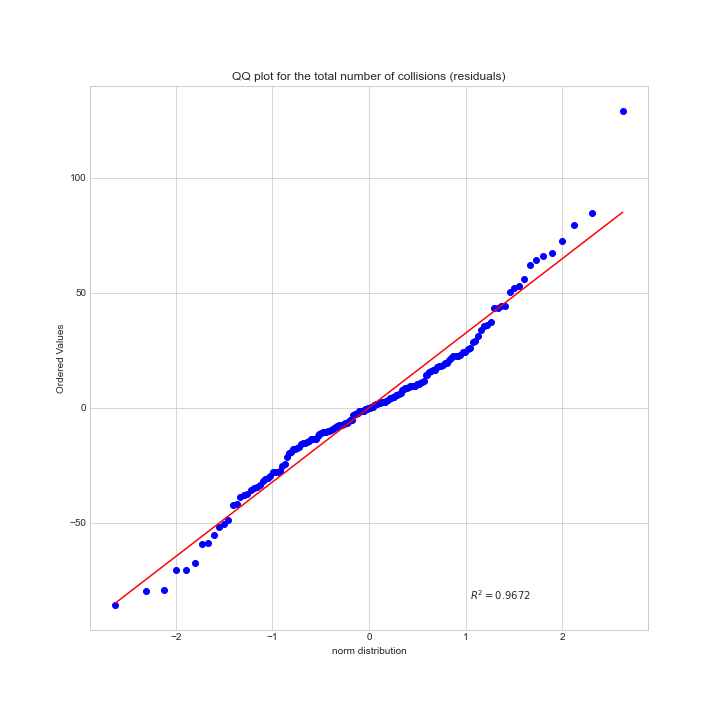
\includegraphics[width=\textwidth]
	{img/lowdensity2kr/assumptions/collisions-norm-fit.png}
	\caption{Normality check for collisions}\label{fig:system}
\end{figure}

\begin{figure}
	\centering
	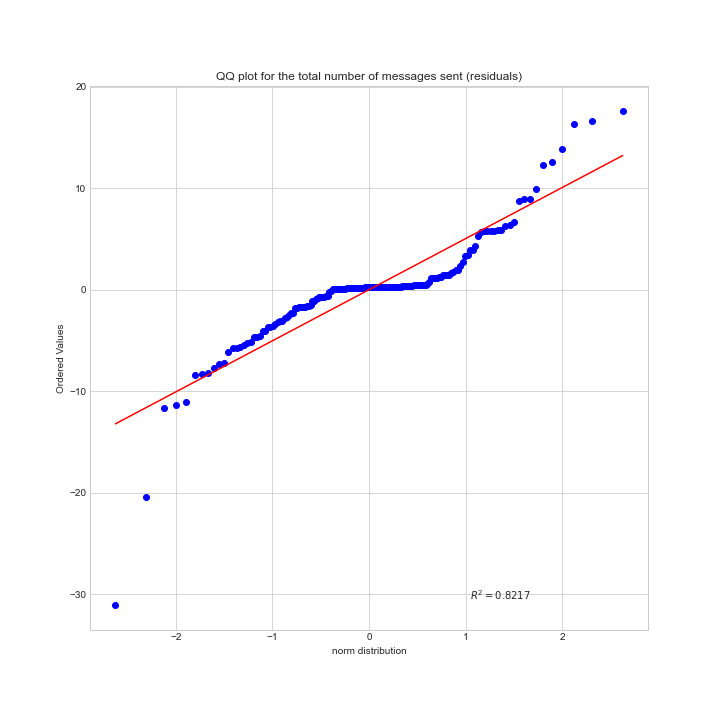
\includegraphics[width=\textwidth]
	{img/lowdensity2kr/assumptions/msgsPerSlot-norm-fit.png}
	\caption{Normality check for messages per slot}\label{fig:system}
\end{figure}

\begin{figure}
	\centering
	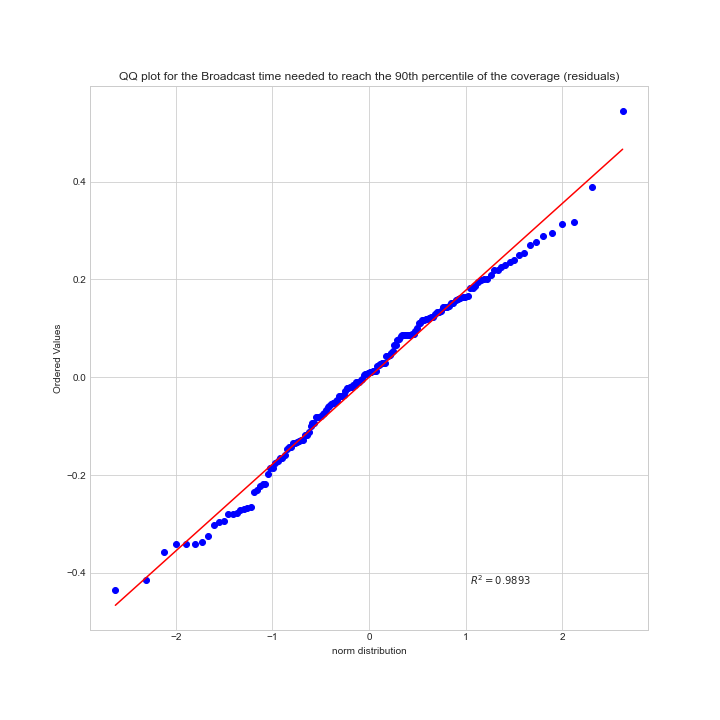
\includegraphics[width=\textwidth]
	{img/lowdensity2kr/assumptions/broadcastTime90-norm-fit.png}
	\caption{Normality check for \(90\%\) broadcast time}\label{fig:system}
\end{figure}

We can see that for all the configurations the assumption is verified, because
the residuals follows the line.  Remember that for the broadcast time, instead
of a linear transformation, we used a lognormal one.

\subsubsection{Constant standard deviation}

For the constant standard deviation assumption, we have to see these
scatterplots:

\begin{figure}
	\centering
	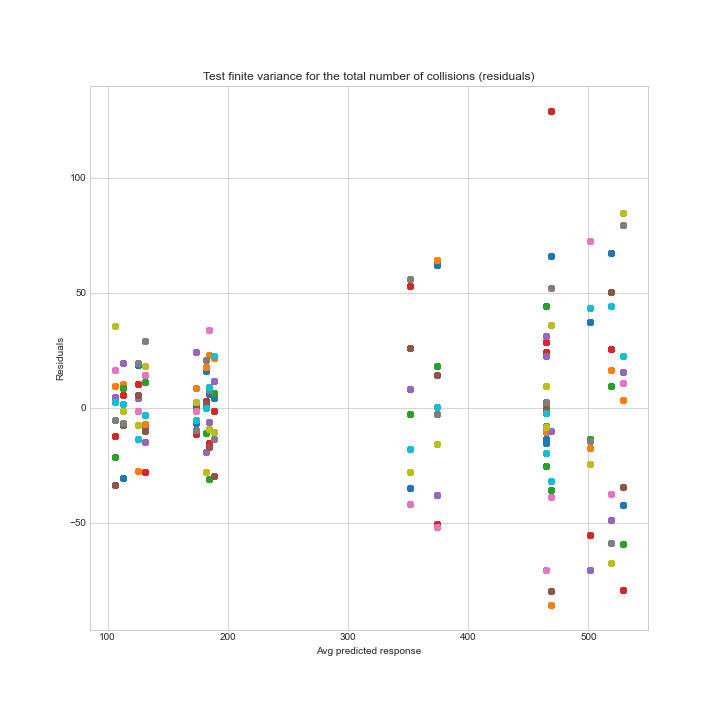
\includegraphics[width=\textwidth]
	{img/lowdensity2kr/assumptions/collisions-variance.png}
	\caption{Constant standard deviation check for
	collisions}\label{fig:system}
\end{figure}

\begin{figure}
	\centering
	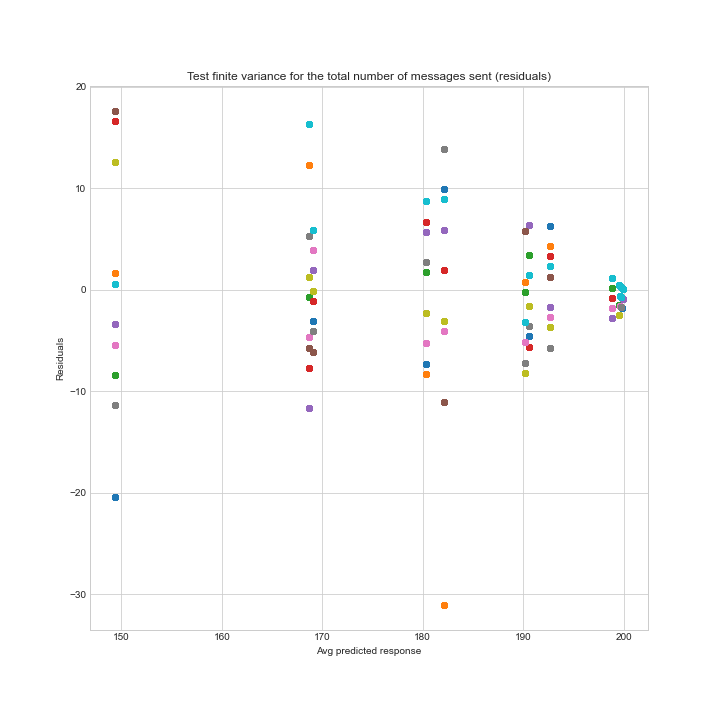
\includegraphics[width=\textwidth]
	{img/lowdensity2kr/assumptions/msgsPerSlot-variance.png}
	\caption{Constant standard deviation check for messages per
	slot}\label{fig:system}
\end{figure}

\begin{figure}
	\centering
	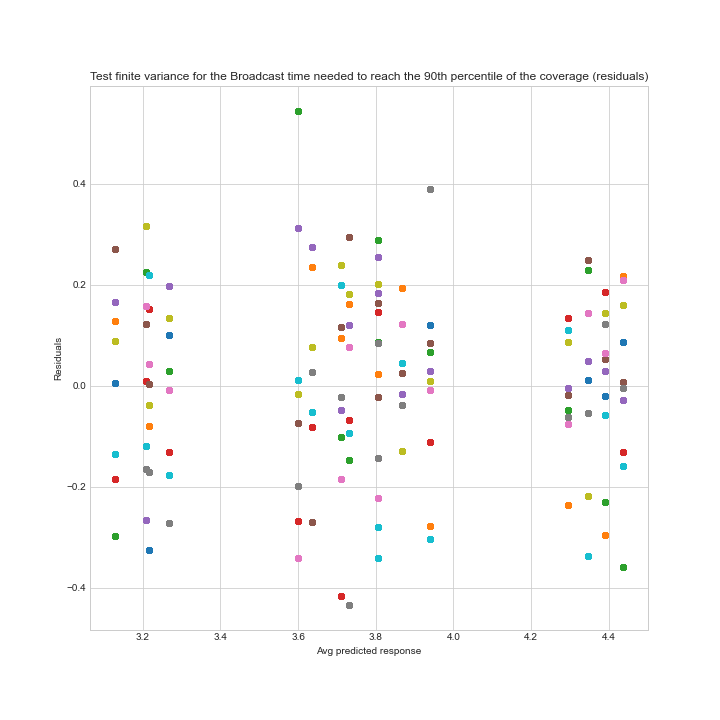
\includegraphics[width=\textwidth]
	{img/lowdensity2kr/assumptions/broadcastTime90-variance.png}
	\caption{Constant standard deviation check for \(90\%\) broadcast
	time}\label{fig:system}
\end{figure}

We can't see trends for every configuration of broadcast time. For collisions
and messages we have respectively increasing and decreasing trend, but residuals
are one order of magnitude low with respect to the predicted values.

After these considerations we can say that the constant standard deviation
assumption is proved.

\subsubsection{IIDness}
For the IID assumption, we have to see these scatterplots:
\begin{figure}
	\centering
	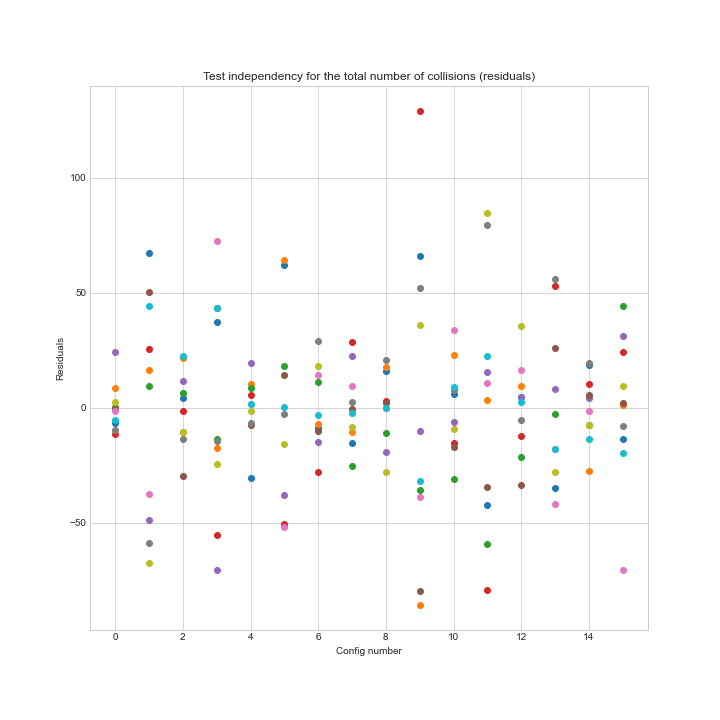
\includegraphics[width=\textwidth]
	{img/lowdensity2kr/assumptions/collisions-independency.png}
	\caption{Constant standard deviation check for
	collisions}\label{fig:system}
\end{figure}

\begin{figure}
	\centering
	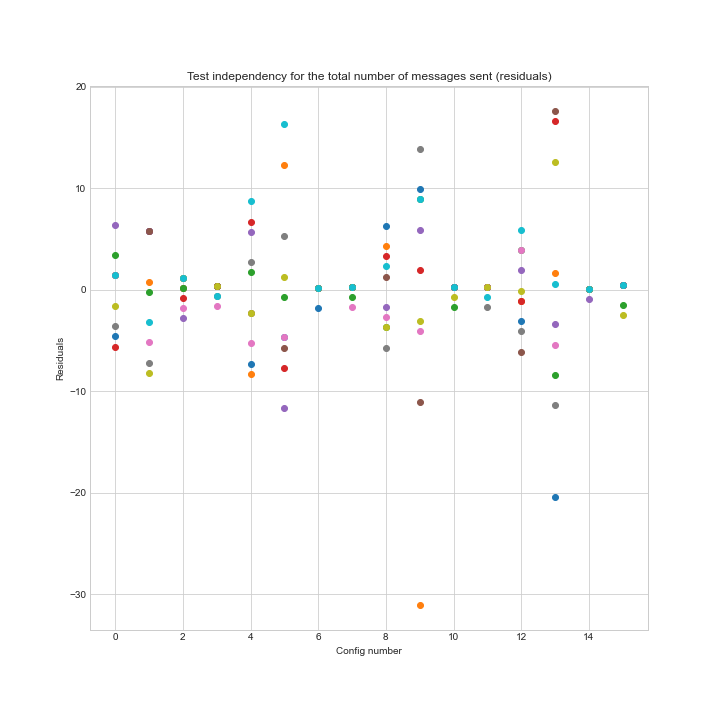
\includegraphics[width=\textwidth]
	{img/lowdensity2kr/assumptions/msgsPerSlot-independency.png}
	\caption{Constant standard deviation check for messages per
	slot}\label{fig:system}
\end{figure}

\begin{figure}
	\centering
	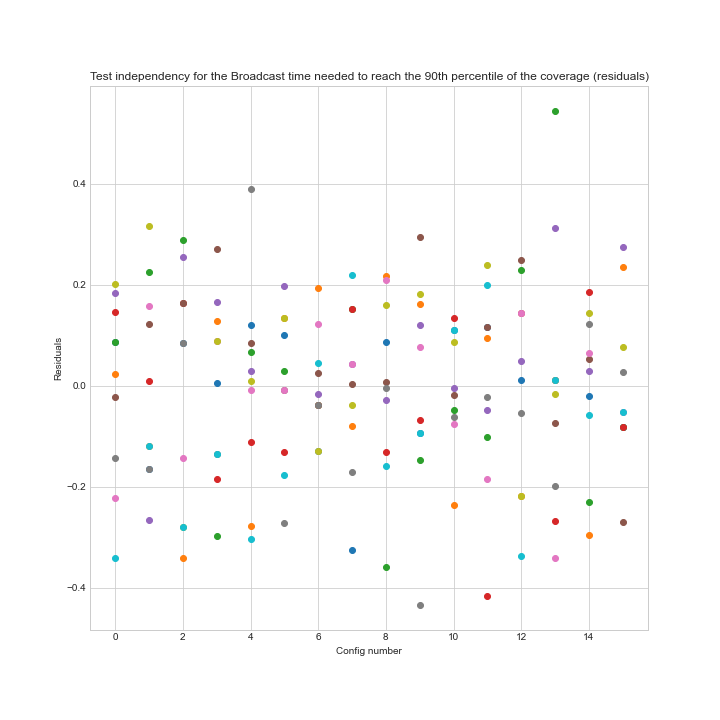
\includegraphics[width=\textwidth]
	{img/lowdensity2kr/assumptions/broadcastTime90-independency.png}
	\caption{Constant standard deviation check for \(90\%\) broadcast
	time}\label{fig:system}
\end{figure}

No one of these scatterplots show a trend, so also the IID assumption is
verified.
